\documentclass[1p]{elsarticle_modified}
%\bibliographystyle{elsarticle-num}

%\usepackage[colorlinks]{hyperref}
%\usepackage{abbrmath_seonhwa} %\Abb, \Ascr, \Acal ,\Abf, \Afrak
\usepackage{amsfonts}
\usepackage{amssymb}
\usepackage{amsmath}
\usepackage{amsthm}
\usepackage{scalefnt}
\usepackage{amsbsy}
\usepackage{kotex}
\usepackage{caption}
\usepackage{subfig}
\usepackage{color}
\usepackage{graphicx}
\usepackage{xcolor} %% white, black, red, green, blue, cyan, magenta, yellow
\usepackage{float}
\usepackage{setspace}
\usepackage{hyperref}

\usepackage{tikz}
\usetikzlibrary{arrows}

\usepackage{multirow}
\usepackage{array} % fixed length table
\usepackage{hhline}

%%%%%%%%%%%%%%%%%%%%%
\makeatletter
\renewcommand*\env@matrix[1][\arraystretch]{%
	\edef\arraystretch{#1}%
	\hskip -\arraycolsep
	\let\@ifnextchar\new@ifnextchar
	\array{*\c@MaxMatrixCols c}}
\makeatother %https://tex.stackexchange.com/questions/14071/how-can-i-increase-the-line-spacing-in-a-matrix
%%%%%%%%%%%%%%%

\usepackage[normalem]{ulem}

\newcommand{\msout}[1]{\ifmmode\text{\sout{\ensuremath{#1}}}\else\sout{#1}\fi}
%SOURCE: \msout is \stkout macro in https://tex.stackexchange.com/questions/20609/strikeout-in-math-mode

\newcommand{\cancel}[1]{
	\ifmmode
	{\color{red}\msout{#1}}
	\else
	{\color{red}\sout{#1}}
	\fi
}

\newcommand{\add}[1]{
	{\color{blue}\uwave{#1}}
}

\newcommand{\replace}[2]{
	\ifmmode
	{\color{red}\msout{#1}}{\color{blue}\uwave{#2}}
	\else
	{\color{red}\sout{#1}}{\color{blue}\uwave{#2}}
	\fi
}

\newcommand{\Sol}{\mathcal{S}} %segment
\newcommand{\D}{D} %diagram
\newcommand{\A}{\mathcal{A}} %arc


%%%%%%%%%%%%%%%%%%%%%%%%%%%%%5 test

\def\sl{\operatorname{\textup{SL}}(2,\Cbb)}
\def\psl{\operatorname{\textup{PSL}}(2,\Cbb)}
\def\quan{\mkern 1mu \triangleright \mkern 1mu}

\theoremstyle{definition}
\newtheorem{thm}{Theorem}[section]
\newtheorem{prop}[thm]{Proposition}
\newtheorem{lem}[thm]{Lemma}
\newtheorem{ques}[thm]{Question}
\newtheorem{cor}[thm]{Corollary}
\newtheorem{defn}[thm]{Definition}
\newtheorem{exam}[thm]{Example}
\newtheorem{rmk}[thm]{Remark}
\newtheorem{alg}[thm]{Algorithm}

\newcommand{\I}{\sqrt{-1}}
\begin{document}

%\begin{frontmatter}
%
%\title{Boundary parabolic representations of knots up to 8 crossings}
%
%%% Group authors per affiliation:
%\author{Yunhi Cho} 
%\address{Department of Mathematics, University of Seoul, Seoul, Korea}
%\ead{yhcho@uos.ac.kr}
%
%
%\author{Seonhwa Kim} %\fnref{s_kim}}
%\address{Center for Geometry and Physics, Institute for Basic Science, Pohang, 37673, Korea}
%\ead{ryeona17@ibs.re.kr}
%
%\author{Hyuk Kim}
%\address{Department of Mathematical Sciences, Seoul National University, Seoul 08826, Korea}
%\ead{hyukkim@snu.ac.kr}
%
%\author{Seokbeom Yoon}
%\address{Department of Mathematical Sciences, Seoul National University, Seoul, 08826,  Korea}
%\ead{sbyoon15@snu.ac.kr}
%
%\begin{abstract}
%We find all boundary parabolic representation of knots up to 8 crossings.
%
%\end{abstract}
%\begin{keyword}
%    \MSC[2010] 57M25 
%\end{keyword}
%
%\end{frontmatter}

%\linenumbers
%\tableofcontents
%
\newcommand\colored[1]{\textcolor{white}{\rule[-0.35ex]{0.8em}{1.4ex}}\kern-0.8em\color{red} #1}%
%\newcommand\colored[1]{\textcolor{white}{ #1}\kern-2.17ex	\textcolor{white}{ #1}\kern-1.81ex	\textcolor{white}{ #1}\kern-2.15ex\color{red}#1	}

{\Large $\underline{10_{54}~(K10a_{48})}$}

\setlength{\tabcolsep}{10pt}
\renewcommand{\arraystretch}{1.6}
\vspace{1cm}\begin{tabular}{m{100pt}>{\centering\arraybackslash}m{274pt}}
\multirow{5}{120pt}{
	\centering
	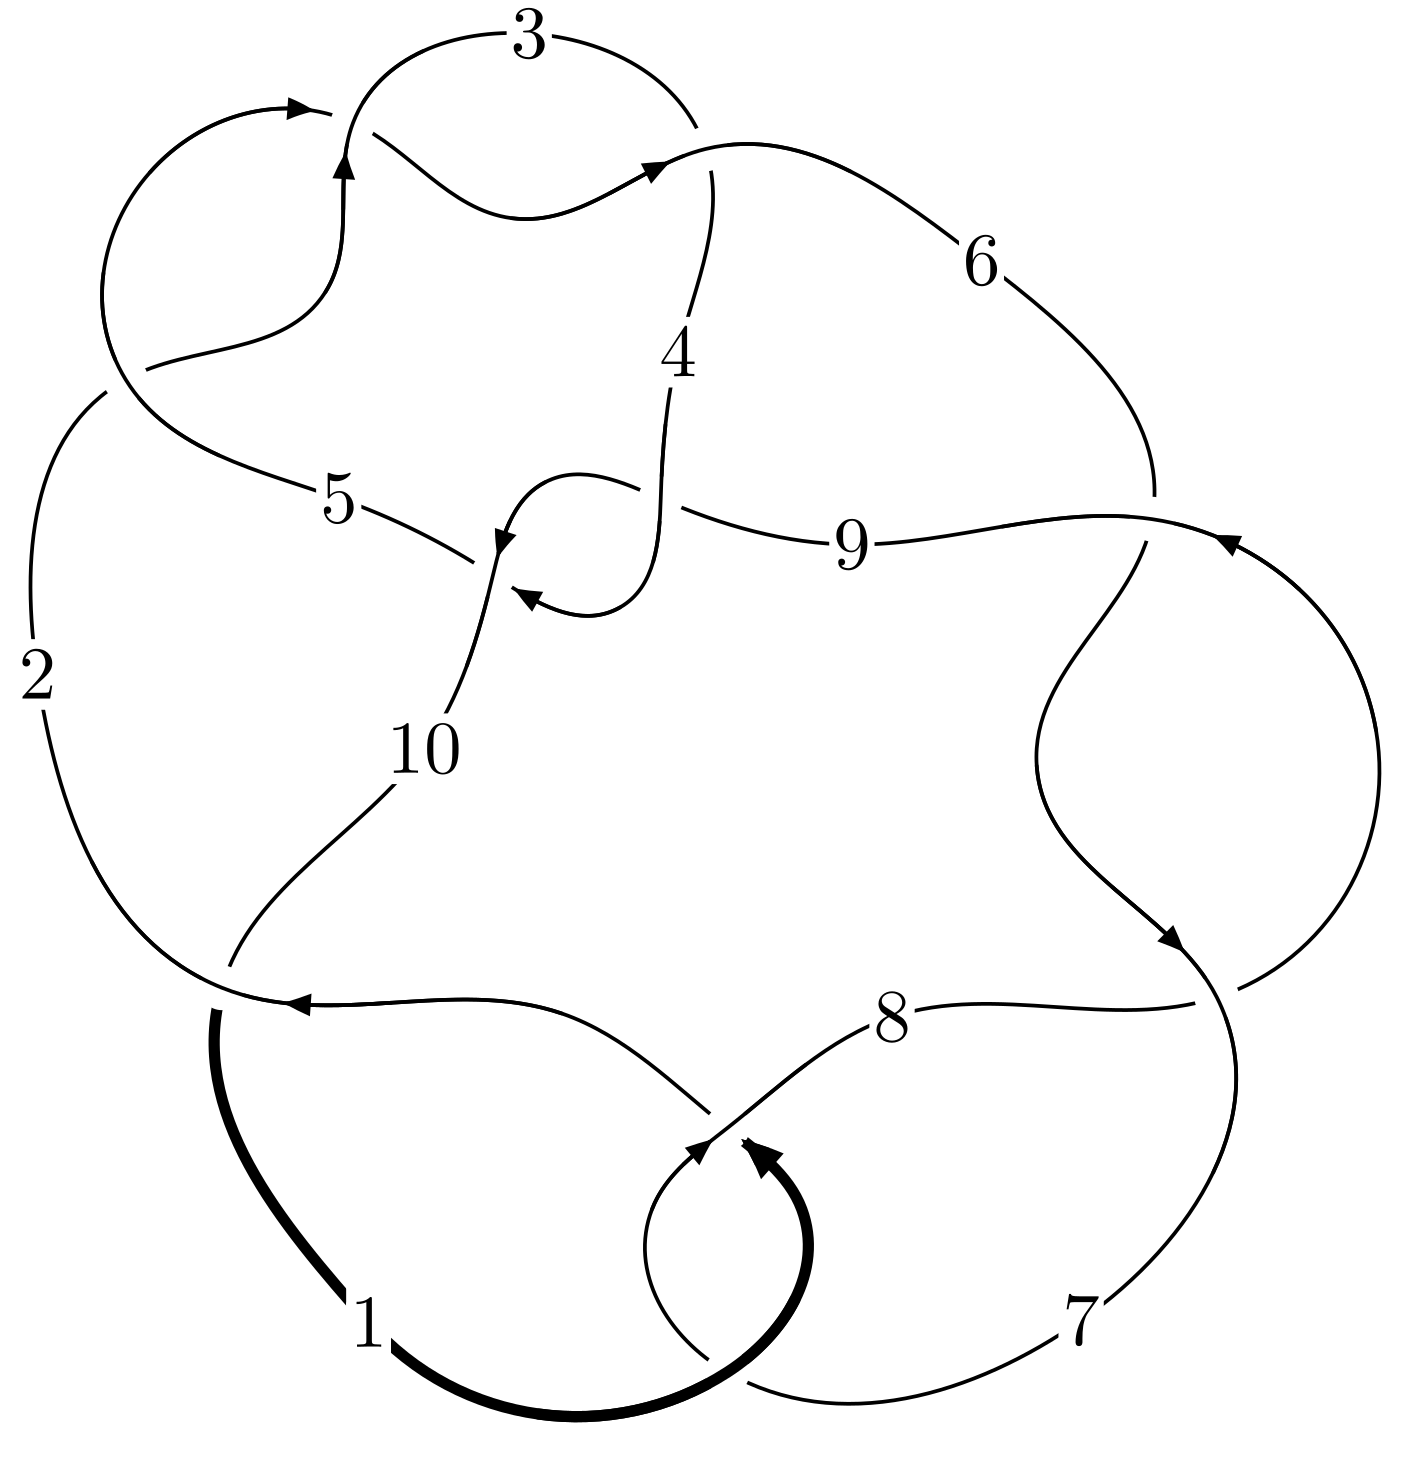
\includegraphics[width=112pt]{../../../GIT/diagram.site/Diagrams/png/138_10_54.png}\\
\ \ \ A knot diagram\footnotemark}&
\allowdisplaybreaks
\textbf{Linearized knot diagam} \\
\cline{2-2}
 &
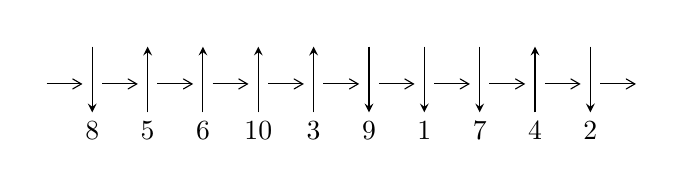
\begin{tikzpicture}[x=20pt, y=17pt]
	% nodes
	\node (C0) at (0, 0) {};
	\node (C1) at (1, 0) {};
	\node (C1U) at (1, +1) {};
	\node (C1D) at (1, -1) {8};

	\node (C2) at (2, 0) {};
	\node (C2U) at (2, +1) {};
	\node (C2D) at (2, -1) {5};

	\node (C3) at (3, 0) {};
	\node (C3U) at (3, +1) {};
	\node (C3D) at (3, -1) {6};

	\node (C4) at (4, 0) {};
	\node (C4U) at (4, +1) {};
	\node (C4D) at (4, -1) {10};

	\node (C5) at (5, 0) {};
	\node (C5U) at (5, +1) {};
	\node (C5D) at (5, -1) {3};

	\node (C6) at (6, 0) {};
	\node (C6U) at (6, +1) {};
	\node (C6D) at (6, -1) {9};

	\node (C7) at (7, 0) {};
	\node (C7U) at (7, +1) {};
	\node (C7D) at (7, -1) {1};

	\node (C8) at (8, 0) {};
	\node (C8U) at (8, +1) {};
	\node (C8D) at (8, -1) {7};

	\node (C9) at (9, 0) {};
	\node (C9U) at (9, +1) {};
	\node (C9D) at (9, -1) {4};

	\node (C10) at (10, 0) {};
	\node (C10U) at (10, +1) {};
	\node (C10D) at (10, -1) {2};
	\node (C11) at (11, 0) {};

	% arrows
	\draw[->,>={angle 60}]
	(C0) edge (C1) (C1) edge (C2) (C2) edge (C3) (C3) edge (C4) (C4) edge (C5) (C5) edge (C6) (C6) edge (C7) (C7) edge (C8) (C8) edge (C9) (C9) edge (C10) (C10) edge (C11) ;	\draw[->,>=stealth]
	(C1U) edge (C1D) (C2D) edge (C2U) (C3D) edge (C3U) (C4D) edge (C4U) (C5D) edge (C5U) (C6U) edge (C6D) (C7U) edge (C7D) (C8U) edge (C8D) (C9D) edge (C9U) (C10U) edge (C10D) ;
	\end{tikzpicture} \\
\hhline{~~} \\& 
\textbf{Solving Sequence} \\ \cline{2-2} 
 &
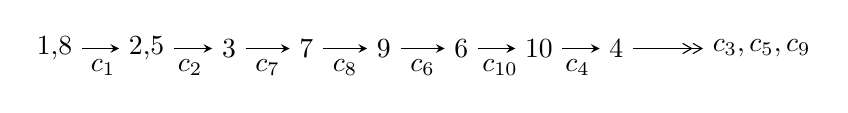
\begin{tikzpicture}[x=28pt, y=7pt]
	% node
	\node (A0) at (-1/8, 0) {1,8};
	\node (A1) at (17/16, 0) {2,5};
	\node (A2) at (17/8, 0) {3};
	\node (A3) at (25/8, 0) {7};
	\node (A4) at (33/8, 0) {9};
	\node (A5) at (41/8, 0) {6};
	\node (A6) at (49/8, 0) {10};
	\node (A7) at (57/8, 0) {4};
	\node (C1) at (1/2, -1) {$c_{1}$};
	\node (C2) at (13/8, -1) {$c_{2}$};
	\node (C3) at (21/8, -1) {$c_{7}$};
	\node (C4) at (29/8, -1) {$c_{8}$};
	\node (C5) at (37/8, -1) {$c_{6}$};
	\node (C6) at (45/8, -1) {$c_{10}$};
	\node (C7) at (53/8, -1) {$c_{4}$};
	\node (A8) at (9, 0) {$c_{3},c_{5},c_{9}$};

	% edge
	\draw[->,>=stealth]	
	(A0) edge (A1) (A1) edge (A2) (A2) edge (A3) (A3) edge (A4) (A4) edge (A5) (A5) edge (A6) (A6) edge (A7) ;
	\draw[->>,>={angle 60}]	
	(A7) edge (A8);
\end{tikzpicture} \\ 

\end{tabular} \\

\footnotetext{
The image of knot diagram is generated by the software ``\textbf{Draw programme}" developed by Andrew Bartholomew(\url{http://www.layer8.co.uk/maths/draw/index.htm\#Running-draw}), where we modified some parts for our purpose(\url{https://github.com/CATsTAILs/LinksPainter}).
}\phantom \\ \newline 
\centering \textbf{Ideals for irreducible components\footnotemark of $X_{\text{par}}$} 
 
\begin{align*}
I^u_{1}&=\langle 
- u^{16}+2 u^{14}-6 u^{12}+8 u^{10}-2 u^9-10 u^8+2 u^7+8 u^6-6 u^5-4 u^4+4 u^3+b-2 u,\;u^{23}+u^{22}+\cdots+a+2,\\
\phantom{I^u_{1}}&\phantom{= \langle  }u^{26}+2 u^{25}+\cdots+2 u-1\rangle \\
I^u_{2}&=\langle 
u^2+b,\;a+u,\;u^3- u^2+1\rangle \\
\\
\end{align*}
\raggedright * 2 irreducible components of $\dim_{\mathbb{C}}=0$, with total 29 representations.\\
\footnotetext{All coefficients of polynomials are rational numbers. But the coefficients are sometimes approximated in decimal forms when there is not enough margin.}
\newpage
\renewcommand{\arraystretch}{1}
\centering \section*{I. $I^u_{1}= \langle - u^{16}+2 u^{14}+\cdots+b-2 u,\;u^{23}+u^{22}+\cdots+a+2,\;u^{26}+2 u^{25}+\cdots+2 u-1 \rangle$}
\flushleft \textbf{(i) Arc colorings}\\
\begin{tabular}{m{7pt} m{180pt} m{7pt} m{180pt} }
\flushright $a_{1}=$&$\begin{pmatrix}1\\0\end{pmatrix}$ \\
\flushright $a_{8}=$&$\begin{pmatrix}0\\u\end{pmatrix}$ \\
\flushright $a_{2}=$&$\begin{pmatrix}1\\u^2\end{pmatrix}$ \\
\flushright $a_{5}=$&$\begin{pmatrix}- u^{23}- u^{22}+\cdots+2 u-2\\u^{16}-2 u^{14}+\cdots-4 u^3+2 u\end{pmatrix}$ \\
\flushright $a_{3}=$&$\begin{pmatrix}- u^{25}- u^{24}+\cdots-2 u+3\\- u^{25}-2 u^{24}+\cdots-4 u+1\end{pmatrix}$ \\
\flushright $a_{7}=$&$\begin{pmatrix}u\\u\end{pmatrix}$ \\
\flushright $a_{9}=$&$\begin{pmatrix}- u^3\\- u^3+u\end{pmatrix}$ \\
\flushright $a_{6}=$&$\begin{pmatrix}u^5+u\\u^5- u^3+u\end{pmatrix}$ \\
\flushright $a_{10}=$&$\begin{pmatrix}- u^2+1\\- u^4\end{pmatrix}$ \\
\flushright $a_{4}=$&$\begin{pmatrix}2 u^{25}+2 u^{24}+\cdots+2 u-3\\2 u^{25}+4 u^{24}+\cdots+7 u-2\end{pmatrix}$\\&\end{tabular}
\flushleft \textbf{(ii) Obstruction class $= -1$}\\~\\
\flushleft \textbf{(iii) Cusp Shapes $= 3 u^{25}+6 u^{24}-4 u^{23}-20 u^{22}+15 u^{21}+67 u^{20}-6 u^{19}-133 u^{18}+9 u^{17}+243 u^{16}+26 u^{15}-312 u^{14}-14 u^{13}+380 u^{12}+8 u^{11}-325 u^{10}+66 u^9+275 u^8-98 u^7-154 u^6+121 u^5+79 u^4-58 u^3-13 u^2+27 u+3$}\\~\\
\newpage\renewcommand{\arraystretch}{1}
\flushleft \textbf{(iv) u-Polynomials at the component}\newline \\
\begin{tabular}{m{50pt}|m{274pt}}
Crossings & \hspace{64pt}u-Polynomials at each crossing \\
\hline $$\begin{aligned}c_{1},c_{7}\end{aligned}$$&$\begin{aligned}
&u^{26}+2 u^{25}+\cdots+2 u-1
\end{aligned}$\\
\hline $$\begin{aligned}c_{2},c_{3},c_{5}\end{aligned}$$&$\begin{aligned}
&u^{26}+4 u^{25}+\cdots- u-1
\end{aligned}$\\
\hline $$\begin{aligned}c_{4},c_{9}\end{aligned}$$&$\begin{aligned}
&u^{26}- u^{25}+\cdots-12 u+8
\end{aligned}$\\
\hline $$\begin{aligned}c_{6},c_{8},c_{10}\end{aligned}$$&$\begin{aligned}
&u^{26}+6 u^{25}+\cdots+14 u+1
\end{aligned}$\\
\hline
\end{tabular}\\~\\
\newpage\renewcommand{\arraystretch}{1}
\flushleft \textbf{(v) Riley Polynomials at the component}\newline \\
\begin{tabular}{m{50pt}|m{274pt}}
Crossings & \hspace{64pt}Riley Polynomials at each crossing \\
\hline $$\begin{aligned}c_{1},c_{7}\end{aligned}$$&$\begin{aligned}
&y^{26}-6 y^{25}+\cdots-14 y+1
\end{aligned}$\\
\hline $$\begin{aligned}c_{2},c_{3},c_{5}\end{aligned}$$&$\begin{aligned}
&y^{26}-28 y^{25}+\cdots+9 y+1
\end{aligned}$\\
\hline $$\begin{aligned}c_{4},c_{9}\end{aligned}$$&$\begin{aligned}
&y^{26}-21 y^{25}+\cdots-272 y+64
\end{aligned}$\\
\hline $$\begin{aligned}c_{6},c_{8},c_{10}\end{aligned}$$&$\begin{aligned}
&y^{26}+30 y^{25}+\cdots-38 y+1
\end{aligned}$\\
\hline
\end{tabular}\\~\\
\newpage\flushleft \textbf{(vi) Complex Volumes and Cusp Shapes}
$$\begin{array}{c|c|c}  
\text{Solutions to }I^u_{1}& \I (\text{vol} + \sqrt{-1}CS) & \text{Cusp shape}\\
 \hline 
\begin{aligned}
u &= \phantom{-}0.846572 + 0.426560 I \\
a &= \phantom{-}0.369102 + 1.145660 I \\
b &= -0.275280 + 0.265581 I\end{aligned}
 & \phantom{-}0.25133 - 3.55563 I & \phantom{-}0.67279 + 7.82227 I \\ \hline\begin{aligned}
u &= \phantom{-}0.846572 - 0.426560 I \\
a &= \phantom{-}0.369102 - 1.145660 I \\
b &= -0.275280 - 0.265581 I\end{aligned}
 & \phantom{-}0.25133 + 3.55563 I & \phantom{-}0.67279 - 7.82227 I \\ \hline\begin{aligned}
u &= -1.05838\phantom{ +0.000000I} \\
a &= \phantom{-}0.930276\phantom{ +0.000000I} \\
b &= -0.383659\phantom{ +0.000000I}\end{aligned}
 & \phantom{-}3.31147\phantom{ +0.000000I} & \phantom{-}2.10670\phantom{ +0.000000I} \\ \hline\begin{aligned}
u &= \phantom{-}1.024210 + 0.483667 I \\
a &= -0.41844 - 1.77157 I \\
b &= -0.06027 - 1.68353 I\end{aligned}
 & \phantom{-}6.23030 - 6.31822 I & \phantom{-}4.39684 + 5.98052 I \\ \hline\begin{aligned}
u &= \phantom{-}1.024210 - 0.483667 I \\
a &= -0.41844 + 1.77157 I \\
b &= -0.06027 + 1.68353 I\end{aligned}
 & \phantom{-}6.23030 + 6.31822 I & \phantom{-}4.39684 - 5.98052 I \\ \hline\begin{aligned}
u &= \phantom{-}0.352335 + 0.784080 I \\
a &= -1.72547 - 0.09649 I \\
b &= -0.633711 - 1.002200 I\end{aligned}
 & \phantom{-}8.43955 + 1.72575 I & \phantom{-}8.31886 - 0.55186 I \\ \hline\begin{aligned}
u &= \phantom{-}0.352335 - 0.784080 I \\
a &= -1.72547 + 0.09649 I \\
b &= -0.633711 + 1.002200 I\end{aligned}
 & \phantom{-}8.43955 - 1.72575 I & \phantom{-}8.31886 + 0.55186 I \\ \hline\begin{aligned}
u &= -0.714859 + 0.468666 I \\
a &= \phantom{-}1.90202 - 1.71328 I \\
b &= \phantom{-}0.66236 - 1.66931 I\end{aligned}
 & \phantom{-}2.60764 + 1.82411 I & \phantom{-}3.14672 - 3.41167 I \\ \hline\begin{aligned}
u &= -0.714859 - 0.468666 I \\
a &= \phantom{-}1.90202 + 1.71328 I \\
b &= \phantom{-}0.66236 + 1.66931 I\end{aligned}
 & \phantom{-}2.60764 - 1.82411 I & \phantom{-}3.14672 + 3.41167 I \\ \hline\begin{aligned}
u &= \phantom{-}0.884681 + 0.778751 I \\
a &= -0.886815 - 0.322575 I \\
b &= -0.169423 - 1.226160 I\end{aligned}
 & \phantom{-}3.71424 - 2.93248 I & -1.57920 + 3.07432 I\\
 \hline 
 \end{array}$$\newpage$$\begin{array}{c|c|c}  
\text{Solutions to }I^u_{1}& \I (\text{vol} + \sqrt{-1}CS) & \text{Cusp shape}\\
 \hline 
\begin{aligned}
u &= \phantom{-}0.884681 - 0.778751 I \\
a &= -0.886815 + 0.322575 I \\
b &= -0.169423 + 1.226160 I\end{aligned}
 & \phantom{-}3.71424 + 2.93248 I & -1.57920 - 3.07432 I \\ \hline\begin{aligned}
u &= -0.782649 + 0.135062 I \\
a &= -0.896199 + 0.591232 I \\
b &= -0.443229 + 0.258658 I\end{aligned}
 & -1.320760 + 0.339413 I & -6.54496 - 0.64162 I \\ \hline\begin{aligned}
u &= -0.782649 - 0.135062 I \\
a &= -0.896199 - 0.591232 I \\
b &= -0.443229 - 0.258658 I\end{aligned}
 & -1.320760 - 0.339413 I & -6.54496 + 0.64162 I \\ \hline\begin{aligned}
u &= -0.890496 + 0.876738 I \\
a &= \phantom{-}0.197188 - 0.399123 I \\
b &= \phantom{-}0.018430 - 1.188940 I\end{aligned}
 & \phantom{-}8.31406 + 0.26926 I & \phantom{-}5.67547 + 0.24692 I \\ \hline\begin{aligned}
u &= -0.890496 - 0.876738 I \\
a &= \phantom{-}0.197188 + 0.399123 I \\
b &= \phantom{-}0.018430 + 1.188940 I\end{aligned}
 & \phantom{-}8.31406 - 0.26926 I & \phantom{-}5.67547 - 0.24692 I \\ \hline\begin{aligned}
u &= -0.851371 + 0.929645 I \\
a &= -1.80201 + 0.27660 I \\
b &= -0.91806 + 3.09384 I\end{aligned}
 & \phantom{-}15.7394 - 4.0044 I & \phantom{-}7.52896 + 1.00327 I \\ \hline\begin{aligned}
u &= -0.851371 - 0.929645 I \\
a &= -1.80201 - 0.27660 I \\
b &= -0.91806 - 3.09384 I\end{aligned}
 & \phantom{-}15.7394 + 4.0044 I & \phantom{-}7.52896 - 1.00327 I \\ \hline\begin{aligned}
u &= \phantom{-}0.920092 + 0.872965 I \\
a &= \phantom{-}2.37362 + 0.94576 I \\
b &= \phantom{-}0.20685 + 3.87193 I\end{aligned}
 & \phantom{-}10.46160 - 3.23113 I & \phantom{-}6.21855 + 2.44261 I \\ \hline\begin{aligned}
u &= \phantom{-}0.920092 - 0.872965 I \\
a &= \phantom{-}2.37362 - 0.94576 I \\
b &= \phantom{-}0.20685 - 3.87193 I\end{aligned}
 & \phantom{-}10.46160 + 3.23113 I & \phantom{-}6.21855 - 2.44261 I \\ \hline\begin{aligned}
u &= -0.942244 + 0.855193 I \\
a &= \phantom{-}1.174670 - 0.368934 I \\
b &= \phantom{-}0.172482 - 1.056320 I\end{aligned}
 & \phantom{-}8.15003 + 6.14753 I & \phantom{-}5.18996 - 5.20017 I\\
 \hline 
 \end{array}$$\newpage$$\begin{array}{c|c|c}  
\text{Solutions to }I^u_{1}& \I (\text{vol} + \sqrt{-1}CS) & \text{Cusp shape}\\
 \hline 
\begin{aligned}
u &= -0.942244 - 0.855193 I \\
a &= \phantom{-}1.174670 + 0.368934 I \\
b &= \phantom{-}0.172482 + 1.056320 I\end{aligned}
 & \phantom{-}8.15003 - 6.14753 I & \phantom{-}5.18996 + 5.20017 I \\ \hline\begin{aligned}
u &= -0.996075 + 0.858678 I \\
a &= -1.86455 + 1.56620 I \\
b &= \phantom{-}0.61540 + 3.28212 I\end{aligned}
 & \phantom{-}15.2731 + 10.5913 I & \phantom{-}6.79989 - 5.68919 I \\ \hline\begin{aligned}
u &= -0.996075 - 0.858678 I \\
a &= -1.86455 - 1.56620 I \\
b &= \phantom{-}0.61540 - 3.28212 I\end{aligned}
 & \phantom{-}15.2731 - 10.5913 I & \phantom{-}6.79989 + 5.68919 I \\ \hline\begin{aligned}
u &= \phantom{-}0.493543 + 0.417386 I \\
a &= -0.243260 - 0.166657 I \\
b &= \phantom{-}0.698144 + 0.266835 I\end{aligned}
 & \phantom{-}1.336670 + 0.113896 I & \phantom{-}6.51816 + 0.27618 I \\ \hline\begin{aligned}
u &= \phantom{-}0.493543 - 0.417386 I \\
a &= -0.243260 + 0.166657 I \\
b &= \phantom{-}0.698144 - 0.266835 I\end{aligned}
 & \phantom{-}1.336670 - 0.113896 I & \phantom{-}6.51816 - 0.27618 I \\ \hline\begin{aligned}
u &= \phantom{-}0.370909\phantom{ +0.000000I} \\
a &= -1.28999\phantom{ +0.000000I} \\
b &= \phantom{-}0.636266\phantom{ +0.000000I}\end{aligned}
 & \phantom{-}1.14285\phantom{ +0.000000I} & \phantom{-}10.2090\phantom{ +0.000000I}\\
 \hline 
 \end{array}$$\newpage\newpage\renewcommand{\arraystretch}{1}
\centering \section*{II. $I^u_{2}= \langle u^2+b,\;a+u,\;u^3- u^2+1 \rangle$}
\flushleft \textbf{(i) Arc colorings}\\
\begin{tabular}{m{7pt} m{180pt} m{7pt} m{180pt} }
\flushright $a_{1}=$&$\begin{pmatrix}1\\0\end{pmatrix}$ \\
\flushright $a_{8}=$&$\begin{pmatrix}0\\u\end{pmatrix}$ \\
\flushright $a_{2}=$&$\begin{pmatrix}1\\u^2\end{pmatrix}$ \\
\flushright $a_{5}=$&$\begin{pmatrix}- u\\- u^2\end{pmatrix}$ \\
\flushright $a_{3}=$&$\begin{pmatrix}- u+1\\0\end{pmatrix}$ \\
\flushright $a_{7}=$&$\begin{pmatrix}u\\u\end{pmatrix}$ \\
\flushright $a_{9}=$&$\begin{pmatrix}- u^2+1\\- u^2+u+1\end{pmatrix}$ \\
\flushright $a_{6}=$&$\begin{pmatrix}-1\\- u^2\end{pmatrix}$ \\
\flushright $a_{10}=$&$\begin{pmatrix}- u^2+1\\- u^2+u+1\end{pmatrix}$ \\
\flushright $a_{4}=$&$\begin{pmatrix}- u\\- u^2\end{pmatrix}$\\&\end{tabular}
\flushleft \textbf{(ii) Obstruction class $= 1$}\\~\\
\flushleft \textbf{(iii) Cusp Shapes $= -2 u^2+7 u+2$}\\~\\
\newpage\renewcommand{\arraystretch}{1}
\flushleft \textbf{(iv) u-Polynomials at the component}\newline \\
\begin{tabular}{m{50pt}|m{274pt}}
Crossings & \hspace{64pt}u-Polynomials at each crossing \\
\hline $$\begin{aligned}c_{1}\end{aligned}$$&$\begin{aligned}
&u^3- u^2+1
\end{aligned}$\\
\hline $$\begin{aligned}c_{2},c_{3}\end{aligned}$$&$\begin{aligned}
&(u+1)^3
\end{aligned}$\\
\hline $$\begin{aligned}c_{4},c_{9}\end{aligned}$$&$\begin{aligned}
&u^3
\end{aligned}$\\
\hline $$\begin{aligned}c_{5}\end{aligned}$$&$\begin{aligned}
&(u-1)^3
\end{aligned}$\\
\hline $$\begin{aligned}c_{6},c_{10}\end{aligned}$$&$\begin{aligned}
&u^3- u^2+2 u-1
\end{aligned}$\\
\hline $$\begin{aligned}c_{7}\end{aligned}$$&$\begin{aligned}
&u^3+u^2-1
\end{aligned}$\\
\hline $$\begin{aligned}c_{8}\end{aligned}$$&$\begin{aligned}
&u^3+u^2+2 u+1
\end{aligned}$\\
\hline
\end{tabular}\\~\\
\newpage\renewcommand{\arraystretch}{1}
\flushleft \textbf{(v) Riley Polynomials at the component}\newline \\
\begin{tabular}{m{50pt}|m{274pt}}
Crossings & \hspace{64pt}Riley Polynomials at each crossing \\
\hline $$\begin{aligned}c_{1},c_{7}\end{aligned}$$&$\begin{aligned}
&y^3- y^2+2 y-1
\end{aligned}$\\
\hline $$\begin{aligned}c_{2},c_{3},c_{5}\end{aligned}$$&$\begin{aligned}
&(y-1)^3
\end{aligned}$\\
\hline $$\begin{aligned}c_{4},c_{9}\end{aligned}$$&$\begin{aligned}
&y^3
\end{aligned}$\\
\hline $$\begin{aligned}c_{6},c_{8},c_{10}\end{aligned}$$&$\begin{aligned}
&y^3+3 y^2+2 y-1
\end{aligned}$\\
\hline
\end{tabular}\\~\\
\newpage\flushleft \textbf{(vi) Complex Volumes and Cusp Shapes}
$$\begin{array}{c|c|c}  
\text{Solutions to }I^u_{2}& \I (\text{vol} + \sqrt{-1}CS) & \text{Cusp shape}\\
 \hline 
\begin{aligned}
u &= \phantom{-}0.877439 + 0.744862 I \\
a &= -0.877439 - 0.744862 I \\
b &= -0.215080 - 1.307140 I\end{aligned}
 & \phantom{-}4.66906 - 2.82812 I & \phantom{-}7.71191 + 2.59975 I \\ \hline\begin{aligned}
u &= \phantom{-}0.877439 - 0.744862 I \\
a &= -0.877439 + 0.744862 I \\
b &= -0.215080 + 1.307140 I\end{aligned}
 & \phantom{-}4.66906 + 2.82812 I & \phantom{-}7.71191 - 2.59975 I \\ \hline\begin{aligned}
u &= -0.754878\phantom{ +0.000000I} \\
a &= \phantom{-}0.754878\phantom{ +0.000000I} \\
b &= -0.569840\phantom{ +0.000000I}\end{aligned}
 & \phantom{-}0.531480\phantom{ +0.000000I} & -4.42380\phantom{ +0.000000I}\\
 \hline 
 \end{array}$$\newpage
\newpage\renewcommand{\arraystretch}{1}
\centering \section*{ III. u-Polynomials}
\begin{tabular}{m{50pt}|m{274pt}}
Crossings & \hspace{64pt}u-Polynomials at each crossing \\
\hline $$\begin{aligned}c_{1}\end{aligned}$$&$\begin{aligned}
&(u^3- u^2+1)(u^{26}+2 u^{25}+\cdots+2 u-1)
\end{aligned}$\\
\hline $$\begin{aligned}c_{2},c_{3}\end{aligned}$$&$\begin{aligned}
&((u+1)^3)(u^{26}+4 u^{25}+\cdots- u-1)
\end{aligned}$\\
\hline $$\begin{aligned}c_{4},c_{9}\end{aligned}$$&$\begin{aligned}
&u^3(u^{26}- u^{25}+\cdots-12 u+8)
\end{aligned}$\\
\hline $$\begin{aligned}c_{5}\end{aligned}$$&$\begin{aligned}
&((u-1)^3)(u^{26}+4 u^{25}+\cdots- u-1)
\end{aligned}$\\
\hline $$\begin{aligned}c_{6},c_{10}\end{aligned}$$&$\begin{aligned}
&(u^3- u^2+2 u-1)(u^{26}+6 u^{25}+\cdots+14 u+1)
\end{aligned}$\\
\hline $$\begin{aligned}c_{7}\end{aligned}$$&$\begin{aligned}
&(u^3+u^2-1)(u^{26}+2 u^{25}+\cdots+2 u-1)
\end{aligned}$\\
\hline $$\begin{aligned}c_{8}\end{aligned}$$&$\begin{aligned}
&(u^3+u^2+2 u+1)(u^{26}+6 u^{25}+\cdots+14 u+1)
\end{aligned}$\\
\hline
\end{tabular}\newpage\renewcommand{\arraystretch}{1}
\centering \section*{ IV. Riley Polynomials}
\begin{tabular}{m{50pt}|m{274pt}}
Crossings & \hspace{64pt}Riley Polynomials at each crossing \\
\hline $$\begin{aligned}c_{1},c_{7}\end{aligned}$$&$\begin{aligned}
&(y^3- y^2+2 y-1)(y^{26}-6 y^{25}+\cdots-14 y+1)
\end{aligned}$\\
\hline $$\begin{aligned}c_{2},c_{3},c_{5}\end{aligned}$$&$\begin{aligned}
&((y-1)^3)(y^{26}-28 y^{25}+\cdots+9 y+1)
\end{aligned}$\\
\hline $$\begin{aligned}c_{4},c_{9}\end{aligned}$$&$\begin{aligned}
&y^3(y^{26}-21 y^{25}+\cdots-272 y+64)
\end{aligned}$\\
\hline $$\begin{aligned}c_{6},c_{8},c_{10}\end{aligned}$$&$\begin{aligned}
&(y^3+3 y^2+2 y-1)(y^{26}+30 y^{25}+\cdots-38 y+1)
\end{aligned}$\\
\hline
\end{tabular}
\vskip 2pc
\end{document}